
\section{Предобработка электронных писем Хиллари Клинтон}

Этап предобработки можно разбить на 6 шагов.

\begin{enumerate}

\item На вход поступает множество документов определенных форматов (txt, doc или pdf, как в нашем случае). Выбирается библиотека программного кода в зависимости от формата исходного документа и осуществляется извлечение данных из документа в виде неформатированного текста. Этот шаг уже произведен платформой \textit{Kaggle}. Общее количество электронных писем --- 7945.

\item В текстовом файле, взятом из \textit{Kaggle}, могут быть пропущенные данные (например, в связи с плохим качеством pdf-файла). Такие данные пропускаются и нами не обрабатываются. После осуществления этого шага остается 6742 писем. 

\item Текст каждого электронного письма проходит процесс нормализации --- удаляются знаки препинания, выделяются отдельные слова. После этого каждое слово приводится в нижний регистр. 

На этом шаге для дальнейшего анализа можно посмотреть на различного рода статистики.
Ниже приведена гистограмма распределения количества слов каждой длины: 

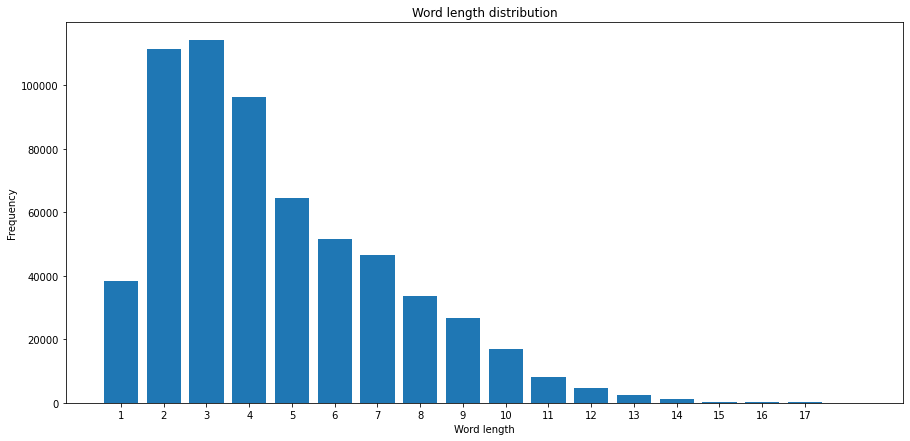
\includegraphics[scale=0.5]{pics/word_lengths.png}

А ниже приведена гистограмма распределения количества электронных писем каждой длины: 

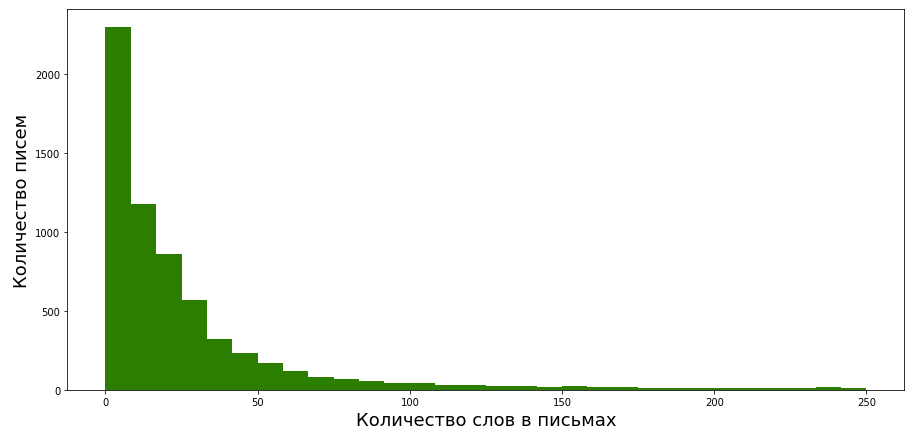
\includegraphics[scale=0.5]{pics/email_lengths.png}

\item Дальше происходит фильтрация текста по стоп-листу --- набору коротких слов (артиклей, предлогов, местоимений), не несущих большой смысловой нагрузки, что приводит к сокращению объема текста и повышению его смысловой ценности. 

\item Следующим шагом происходит лемматизация --- процесс приведения слов к леммам, т. е. нормальным словесным формам. Для реализации лемматизации можно использовать библиотеку программного кода \textit{spaCy} \cite{bib3}, позволяющую привести все слова к нормальной форме. Полученный после выполнения лемматизации набор слов уже может использоваться для проведения машинного обучения и решения конкретных задач. 

\item Индексация --- построение некоторой числовой модели текста, которая переводит текст в удобное для дальнейшей обработки представление. 
 
\end{enumerate}

